\input{preamble}
\usepackage[font=small,labelfont=bf]{caption}  %package for figcap mm.
\raggedbottom
\begin{document}

\frontmatter	% Romertal på de første sider
\input{Chapters/Formalia/Frontpage.tex}
\cleardoublepage		
\input{Chapters/Formalia/titelblad.tex}
\cleardoublepage
\chapter*{Abstract}

In this project an open cluster is simulated using two different algorithms, the fourth order Runge-Kutta and the Velocity Verlet. During the project the fourth order Runge-Kutta is chosen as the main algorithm, as it gives more stable results for a many body system. The evolution of the cluster is studied looking at the energies, the distribution of particles and positions as time progresses. Studying the energies it was found that the system lost energy as particles were ejected from the cluster. When the system reached an approximately equilibrium state after a period of $3\tau_{crunch}$, it was consistent with the virial theorem.

\cleardoublepage	
%\input{Chapters/Formalia/Preface.tex}
%\cleardoublepage			
\tableofcontents*

\mainmatter % Side nummereringen starter ved 1 herfra

	\chapter{Introduction}
This project focuses on numerical simulation of an open cluster using Newtonian gravity. Open clusters contains a few thousand gravitationally bound stars formed as a result of collapse of a molecular cloud. Many of the variable parameters among these stars are constant as they have the same age and same composition and this make them vital in the study of stellar evolution. 

Here two of the finite different methods for solving differential equations namely the fourth order Runge- Kutta method and the Velocity Verlet method are used to develop the code for numerical simulation. At first the stability of these two methods are tested which is important when studying the statistical properties of a system with a large number of particles. This is done by implementing Newtonian two-body problem in three dimension with the two methods and comparing the output from both of them for larger time steps, longer time steps and the time used to advance one time step. Further the system is extended to a cluster containing N particles which is confined inside a sphere of radius in the order of light years. Initially the particles are made to be at rest and using appropriate C++ functions random numbers corresponding to particles masses and positions are generated in such a way that the masses are randomly distributed by a Gaussian distribution around ten solar masses with a standard deviation of one solar mass and the particles are uniformly distributed in the Cartesian coordinates x,y and z within the sphere. 

An estimation of the stability of both the Fourth order Runge Kutta and Velocity Verlet method is made by running the respective codes with gravitational constant G in units of $\tau_{crunch}$, the time period at which the system collapses to a singularity when number of particles tends to infinity and studying the initial and final distribution of particles in the radial direction for time period $\tau_{crunch}$ with different step lengths. The time taken for the system to reach equilibrium is studied for different $\tau_{crunch}$. An analysis of the energy conservation is made by calculating the kinetic and potential energy of the system. 
 


The main part of the report consists of two chapters: The methods and theory chapter, and the results and discussion chapter.
	\chapter{Method}
\label{chap:method} 
The methods introduced in this chapter, are used to study the evolution of bodies, also referred to as particles, in the solar system or in the galaxy. 
Firstly, the fourth order Runge-Kutta method and the Velocity-Verlet method are introduced for a 2-body problem in 3 dimensions, however, since the aim of this project is to investigate the time evolution of a star cluster consisting of $N$ particles, the code is extended to $N$ bodies by incorporating suitable changes. 

To generate the $N$ bodies, a function for generating the position coordinates of the N bodies as uniformly distributed particles within a sphere is introduced as discussed in sec \secref{Method:GeneratingPosMassVel}, along with a function for generating masses that are randomly distributed by a Gaussian distribution around ten solar masses with a standard deviation of one solar mass.

The source codes for the algorithms described in this chapter can be found in the Github folder \url{https://?????}.  \fxnote{fix these lines}


	
\subsection{Transformation between units}

When looking at a planetary system or a larger system like a galaxy it is inconvenient to use the standard units like meters and seconds. So to make it easier to look at how thing are evolving it is better to use days, years, astronomical units or light years.

The gravitational constant in standard units


$ G = 6.67*10^{-11} \frac{\textrm{Nm^2}}{\textrm{kg^2}}$ 
 

For a planetary system like the Earth sun system it is better to look at distance in Astronomical units instead of meters, and use days as a measure of time, as the planet doesn't move much in a second and it would give a to precise measurement also the mass is easier to use if it's in units of solar mass. So to avoid this problem the constants have to be transformed into these unit systems. 

The gravitational constant G is transformed using

$1 AU = 1.495*10^{11} m$ 

$1 M_{sun} = 1.989 * 10 {30} kg$

Then converting the gravitational constant so it can be used in the planetary system

$ G = 2.96* 10^{-4} \frac{\textrm{AU^2}}{days^2m_sun}$ 


So for the star cluster the distances are so great and the time it takes for the stars to move around is quite long, so it is better to use years for time and light years for the distance. 

$Year (yr) = 3.1536*10^7s$

$Light speed (c) = 2.008*10^8 \frac{\textrm{m}}{\textrm{s}}$

$Light year (ly)= 9.45 * 10^15 \textrm{m} $ 

Giving the gravitational constant

$G = 1.536* 10^{-13} \frac{\textrm{ly^2}}{yr^2m_sun}$


	\section{Newtonian two-body problem in three dimension}
\label{Newton2body3D}
The problem of solving the time-evolution of a two-body system in three dimensions can reasonably be considered in two different coordinate systems: one coordinate system with one of the bodies in rest compared to the frame of reference in which the other body is moving, and one coordinate system with both of the bodies moving relative to the frame of reference. 
Both of these reference systems are depicted in \figref{fig:2bodyproblem_coordinatesystems}. 
\begin{figure}[H]
\centering
	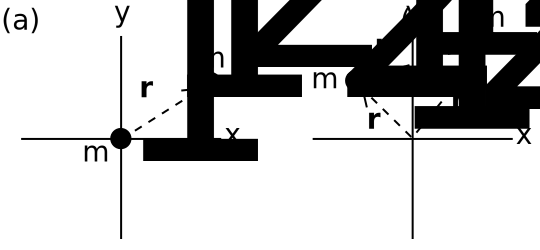
\includegraphics[width=0.6\linewidth]{Figures/2bodyproblem_coordinatesystems.png}
\caption{
Two-dimensional illustration of the three-dimensional problem of determining determining the relative distance and relative velocity between two bodies. 
In (a) body 1 with mass $m_1$ is considered stationary in position- and velocity-space, whilst body 2 with mass $m_2$ moves relative to body 1.
In (b) both body 1 and 2 moves relative to the frame of reference in position and time, yielding that the position vector between body 1 and 2 is given as $\v{r}_{12} = \v{r}_2 - \v{r}_1$.
}
\label{fig:2bodyproblem_coordinatesystems}
\end{figure}
In the codes presented in this section, solving the problem in coordinate system (a) will first be considered for simplicity. Thereafter, the codes will be extended to include the movement of body 1 relative to the coordinate system, since this will be useful when extending the codes to an N body system.  

In the problem, $\v{r}(t)$ is the three-dimensional space vector consisting of the coordinated $(x(t),y(t),z(t))$, whilst $\v{v}(t)$ is the three-dimensional velocity vector with coordinates $(v_x(t),v_y(t),v_z(t))$, both of which are dependent on time. 

In general, the considered differential equation is
\begin{align}
	\frac{dy}{dt} = f(t,y)
	\label{eq:diffEq1}
\end{align}
Which yields that
\begin{align}
	y(t) = \int f(t,y) dt
\end{align}
\fxnote{do we need to write $y_{i+1}$ eq from p. 250 in lecture notes??}
For the two bodies in a three dimensional Newtonian gravitational field this corresponds to six coupled differential equations given by the vector equations
\begin{align}
	\frac{d\v{r}}{dt} = \v{v}
	\qquad \text{and} \qquad
	\frac{d\v{v}}{dt} = - \frac{G M_1 M_2}{r^3} \v{r}
	\label{eq:diffEq2}
\end{align}
\fxnote{maybe we should divide by mass as on p. 248??}
in which $M_1$ and $M_2$ \fxnote{fix the this with $M_1$ and $M_2$} are the masses of the two bodies, respectively, whilst $r$ is the distance between the bodies.
The equations in \eqref{eq:diffEq2} are computed by the script given below in which $drdt$ corresponds to the derivative of the coordinates of the position, and $dvdt$ corresponds to the derivative of the velocity coordinates. 
\begin{lstlisting}
void Derivative(double r[3], double v[3], double (&drdt)[3], double (&dvdt)[3], double G, double mass){
    drdt[0] = v[0];
    drdt[1] = v[1];
    drdt[2] = v[2];

    double distance_squared = r[0]*r[0] + r[1]*r[1] + r[2]*r[2];
    double newtonian_force = -G*mass/pow(distance_squared,1.5);
    dvdt[0] = newtonian_force*r[0];
    dvdt[1] = newtonian_force*r[1];
    dvdt[2] = newtonian_force*r[2];
}
\end{lstlisting}

	\subsection{Velocity-Verlet method}
\label{sec:methodVV}
The basic idea of the Velocity-Verlet algorithm is to write the Taylor expansion of the position in Newton’s equation, one forward step and one backward step in time with step length $\delta t$ as
\begin{align}
	\v{r}(t_i \pm \delta t) = \v{r}(t_i) \pm \v{v} (t_i) \delta t
	+ \v{a} (t_i) \frac{\delta t ^2}{2}  \pm \frac{\delta t ^3}{6} \frac{d^3 \v{r}(t_i)}{dt^3} + \mathcal{O}(\delta t ^4 )
	\label{eq:TaylorExpVVmethod}
\end{align}
in which $\v{v}(t_i) = d\v{r}(t_i)/dt$ is the velocity, and $\v{a}(t_i) = d^2 \v{r}(t_i)/dt^2$ is the acceleration at time $t_i$.
Adding the two expressions in \matref{eq:TaylorExpVVmethod} gives
\begin{align}
	\v{r} (t_i +\delta t) = 2\v{r} (t_i) - \v{r} (t_i -\delta t)  + \v{a} (t_i ) \delta t^2 + \mathcal{O} (\delta t ^4 )
	\label{eq:TaylorExpVVmethod2}
\end{align}
which has a truncation error that goes as $\mathcal{O} (\delta t ^4 )$.
Now, using $\v{r}(t_i-\delta t) = \v{r}(t_i) - \v{v}(t_i) \delta t + \v{a} \delta t^2 /2 + \mathcal{O} (\delta t^3)$, yield that the position at time $t_i+\delta t$ can be determined as 
\begin{align}
	\v{r}(t_i+\delta t) = \v{r}(t_i) + \v{v} (t_i) \delta t + \frac{1}{2} \v{a} (t_i) \delta t^2 
	\label{eq:VVmethodNextPosition}
\end{align}
Since the velocity is not included in \matref{eq:TaylorExpVVmethod2}, it is computed through the Velocity-Verlet scheme where position, velocity and acceleration at time $t_i+\delta t$ is computed from the Taylor expansion as
\begin{align}
	\v{v} (t + \delta t) = \v{v} (t) + \frac{1}{2} ( \v{a} (t) + \v{a} (t + \delta t) ) \delta t
	\label{eq:VVmethodNextVelocity}
\end{align}
The velocity at time $t_i+\delta t$ is in the algorithm computed by first calculating 
\begin{align}
	\v{v}_{part1} (t + \delta t) = \v{v} (t) + \frac{1}{2}  \v{a} (t)  \delta t
	\label{eq:VVmethodNextVelocityPart1}
\end{align}
and then use the \textit{Derivative} function to determine $\v{a} (t + \delta t)$, which is then used to compute the remaining term of \matref{eq:VVmethodNextVelocity} as 
\begin{align}
	\v{v}_{part2} (t + \delta t) = \frac{1}{2} \v{a} (t + \delta t) \delta t
	\label{eq:VVmethodNextVelocityPart2}
\end{align}

The velocity-Verlet method uses the algortihm \textit{Derivative} described in \secref{Newton2body3D}, to generate the six differential equations, in the following while-loop that runs until reaching the final time in time steps of length $\delta t = (t_{initial} - t_{final})/(\# time steps)$.
\begin{lstlisting}
    while(time<=t_final){
    Derivative(r,v,drdt,dvdt,G,mass);
    for(int i=0; i<6 ; i++){
    r[i] = r[i]+dt*drdt[i] + 0.5 * dt * dt * dvdt[i];
    v_partly[i] = drdt[i] + 0.5 * dt * dvdt[i];
    dvdt[i] = v_partly[i];
    }
    Derivative(r,v,drdt,dvdt,G,mass);
    for(int i=0; i<n ; i++){
    v[i] = v_partly[i] + 0.5 * dt * dvdt[i];
    }
    time += dt;
    }
\end{lstlisting}	
	\subsection{Fourth Order Runge-Kutta Method}
\label{sec:methodRK4}
- Remember to write about accuracy of algorithm!!
	\section{Generating Position, Mass and Velocity for Cluster Particles}
\label{Method:GeneratingPosMassVel}
\fxnote{write small intro}
\fxnote{in this section, we can introduce a generation of velocity, if we need that at some point}
\subsection{Gaussian Distributed Mass}
\fxnote{write here, what kind of distribution, we want!}

\begin{lstlisting}
void gaussian_mass_generator(vec (&mass), int number_of_particles)
{
  srand(time(NULL));
  for (int i = 0; i < number_of_particles; i++)
  {
  static int iset = 0;
  static double gset;
  double fac, rsq, v1, v2;
    do{
      v1 = 2.*((double) rand() / (RAND_MAX)) -1.0;
      v2 = 2.*((double) rand() / (RAND_MAX)) -1.0;
      rsq = v1*v1+v2*v2;
    } while (rsq >= 1.0 || rsq == 0.);
    fac = sqrt(-2.*log(rsq)/rsq);
    gset = v1*fac;
    iset = 1;
    mass(i) = v2*fac;
    mass(i) += 10;
  }
}
\end{lstlisting}

\begin{figure}[H]
\centering
	\includegraphics[width=0.7\linewidth]{Figures/random_mass_test.png}
\caption{
Histogram of the mass of 100,000 particles generated by the c++ code introduced \fxnote{where}. 
}
\label{fig:GaussianGeneratedMass}
\end{figure}

\fxnote{eq. include gaussian dist. in fig}

\subsection{Uniformly Distributed Position}
\fxnote{write here, what kind of distribution, we want!}

\begin{lstlisting}
void uniform_pos_generator(mat (&position), int N)
{
double pi=3.14159, c = 2*pi, R = 20;
vec phi(N), r(N), theta(N), x(N), y(N), v(N);

srand(time(NULL));

for (int i=0;i<N;i++){

        x(i) = ((double) rand() / (RAND_MAX)); //random numbers generated in the interval(0,1)
        y(i) = ((double) rand() / (RAND_MAX));
        v(i) = ((double) rand() / (RAND_MAX));
   }
for (int i=0;i<N;i++){
        phi(i)=c*x(i);
        r(i)=R*pow(y(i),1.0/3.0);
        theta(i)=acos(1.0-2.0*v(i));
        position(i,0)=r(i)*sin(theta(i))*cos(phi(i));
        position(i,1)=r(i)*sin(theta(i))*sin(phi(i));
        position(i,2)= r(i)*cos(theta(i));
   }
}
\end{lstlisting}

To test whether the generated positions within the sphere of radius $20$ ly, the density of particles in the cross-sectional area of each $x$-value is determined and plotted as a histogram in \figref{fig:UniformlyGeneratedPos} for $100,000$ particles with position generated by the introduced lines of code.  
The density of particles in the cross-sectional area of each $x$-value is found by dividing the total number of particles with that $x$-value with the cross-sectional area of the sphere in that $x$-value (see \figref{Cross_sectional_area}).
\begin{figure}[H]
\centering
	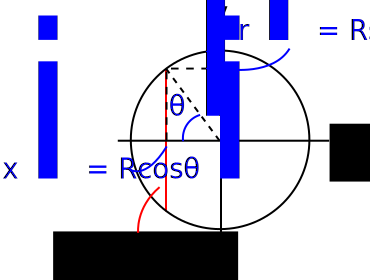
\includegraphics[width=0.4\linewidth]{Figures/Cross_sectional_area.png}
\caption{
Two-dimensional illustration of the three-dimensional problem of determining the density of particles in each $x$-value.
}
\label{fig:Cross_sectional_area}
\end{figure}
The cross-sectional area of the sphere in a specific area is found from a little trigonometry, by first considering that the radius of the circle that makes of the cross-sectional area in a point $x_i$ is given by $r_i = 20sin\theta_i$ ly.  
This yields that the area $A_i$ of the cross-sectional area, in ly, is given as
\begin{align}
	A_i = 400\pi sin^2 \theta_i =  400\pi (1 - cos^2 \theta)
\end{align}
in which the last equal sign stems from $1 = cos^2 \theta + sin^2 \theta$.
But $x_i = 20 cos \theta_i$ ly, giving
\begin{align}
	A_i = \pi (400 - x_i^2)
\end{align}
\begin{figure}[H]
\centering
	\includegraphics[width=0.7\linewidth]{Figures/random_uniform_position_test.png}
\caption{
Histogram of density of 100,000 particles with position generated by the code introduced in \fxnote{where??} as a function of the $x$-coordinate of the particles. The histogram is made with bins in the interval [$-19.5;19.5$] and a bin-size of $0.5$. The distance $x = \pm 20$ from the cluster center is not considered, since the cross-sectional area in that point is zero.
}
\label{fig:UniformlyGeneratedPos}
\end{figure}
	\section{Computing the Energy}
\label{sec:ComputingEnergy}
In order to test whether the energy is conserved, the initial energy of the system can be calculated and printed together with the final energy after a specific time interval.
According to the conservation of energy, these are equal. 

The total energy $E_{tot}$ of the system is found by summing up the potential energy $E_{pot}$ and kinetic energy $E_{kin}$ of the $N$ bodies that constitutes the system.
The total potential energy is calculated as 
\begin{align}
	E_{pot} = \sum _{1=0} ^N \sum _{j \neq i} \frac{m_i m_j}{r_{ij}}
\end{align}
in which $m_i$ and $m_j$ are the masses of the $i$'th and $j$'th body, respectively, $r_{ij} = | \v{r}_i - \v{r}_j |$ is the distance between the two bodies, and $G$ is the gravitational constant. 
The total kinetic energy of the system is calculated as 
\begin{align}
	E_{kin} = \frac{1}{2} \sum _{1=0} ^N m_i v_i ^2
\end{align}
with $v_i$ being the speed of the $i$'th particle calculated as 
$v_i = \sqrt{v_{ix}^2 +v_{iy}^2 +v_{iz}^2}$, and $m_i$ is the corresponding mass of that body. 

The c++ code for computing the total energy of the system is given here below.
When the kinetic energy is calculated, $v_i$ is not explicitly calculated. Instead $v_i^2$ is calculated to reduce the number of floating point operations. 
\begin{lstlisting}
for (int i=0; i<number_of_particles; i++){
	for (int k=0; k<3; k++){
    	kin_en(i) += v(i,k)*v(i,k);
    }
    kin_en(i) = 0.5*m(i)*kin_en(i);
    for (int j=0; j<number_of_particles; j++){
        if (j != i){
        	pot_en(i) += pow(distance_between_particles(i,j),-1.0)*m(j);
        }
    }
    pot_en(i) = pot_en(i)*G*m(i);
    tot_en(i) = kin_en(i)+pot_en(i);
}
\end{lstlisting}

	\chapter{Results and Discussion}
\label{chap:Results}


The results from running the codes described in \chapref{chap:method} for computing the blah blah blah ?? can be found in the GitHub folder  \url{https:/??}, together with the MatLab scripts for the plots presented in this chapter. \fxnote{fix these lines}

	\section{Stability of the 2-body System using Runge-Kutta and Velocity-Verlet}
\label{sec:stability2bodysystem}
The considered two-body system consists of an Earth-like body that orbits a Sun-like body at an initial distance of 1 AU. 
The initial velocity is chosen so that the orbital period of the Earth-like body is 365 days, and due to the choice of the initial position of the Earth-like body relative to the Sun-like body and the initial direction of the velocity of the Earth-like body, the orbit of the Earth-like body is purely in the $x-y$-plane.
Two cases are considered: the situation when the Sun is at rest compared to the frame of reference at all times, and the situation with both the Sun and the Earth moving relative to the frame of reference.
The chosen position and velocity vectors for the Earth and Sun in these two situations are shown in \tabref{tab:SunEarthMarsTest}. 
\begin{table}[H]
\centering
\caption{
Initial position and velocity for Earth and Sun in the Sun-Earth-like two-body system. 
F1 refers to the frame of reference at which the Sun is at rest in origo at all times, whilst F2 refers to the frame of reference in which both the Sun and the Earth moves relative to the coordinate axis. 
The mass of the Earth is given in solar masses, that is $\textrm{M}_E = 3.0\times 10^{-6} \textrm{M}_{\odot}$, and the gravitational constant is given is $2.96\cdot 10^{-4} \frac{\textrm{AU}^2}{\textrm{days}^2 \textrm{M}_{\odot}}$ (see \secref{sec:Conversion}).
}
\begin{center}
\begin{tabular}{ | c | c | c |  }
  \hline			
   &  $\v{r}_{initial}$ [AU] & $\v{v}_{initial}$ [AU/day]  
  \\ \hline
  Earth (F1) & $(1.0,0.0,0.0)$ & $(0.0,0.017,0.0)$
  \\ \hline
  Sun (F2) & $(1.0,1.0,1.0)$  & $(0.0,0.0,0.0)$ 
  \\ \hline
  Earth (F2)  & $(2.0,1.0,1.0)$ & $(0.0,0.017,0.0)$
  \\ \hline
\end{tabular}
\end{center}
\label{tab:SunEarthMarsTest}
\end{table}
\figref{fig:SunEarthMarsTest} shows the final distance between the two bodies as a function of time step length for the two situations: one in which sun is stationary relative to frame of reference and another in which sun is moving relative to the frame of reference. 
In both cases the final distance after 100 years is calculated between the Sun- and the Earth-like bodies and plotted as a function of length of time steps using both the fourth order Runga Kutta method and the Velocity-Verlet method. 
\begin{figure}[H]
\centering
\begin{minipage}{.5\textwidth}
  \centering
  \includegraphics[width=1\linewidth]{Figures/Test_2body_system_earth.png}
\end{minipage}%
\begin{minipage}{.5\textwidth}
  \centering
  \includegraphics[width=1\linewidth]{Figures/Test_2body_system_earth_sun.png}
\end{minipage}
\caption{
Distance between bodies after 100 years as a function of time step length for the Earth-Sun-like two-body system using both the forth order Runge-Kutta method and the Velocity-Verlet method. 
The leftmost plot do not allow for Sun motion relative to the frame of reference, whilst the rightmost allows for movement of both the Earth and the Sun relative to the frame of reference.
}
\label{fig:SunEarthMarsTest}
\end{figure}
The result using the Velocity-Verlet method shows a gradual increase in the final distance between the two bodies after 100 years, as the length of time steps increases, whereas the final distance after 100 years gained by the fourth order Runga-Kutta method shows fluctuations for shorter time step lengths, which is slightly more when sun is stationary relative to the frame of reference.
As time step length reaches about 10 days, the distance, determined by the Runge-Kutta method, between the two bodies decreases, and the final distance after 100 years between the Earth-like body and the Sun-like body starts varying a lot with a change in time step length, meaning that the Runge-Kutta method is very unstable for large time steps, greater than approximately 10 days for this situation.
However, both the Velocity-Verlet and forth order Runge-Kutta method seems to have stabilized for time steps smaller than or equal to 5 days, both for the situation with a stationary Sun and for the situation with both the Sun and Earth moving relative to the coordinate system.
Hence, the time step length of 5 days is used to study the stability of the two methods for long time periods in \figref{fig:SunEarthMarsTest2}.
\begin{figure}[H]
\centering
\begin{minipage}{.5\textwidth}
  \centering
  \includegraphics[width=1\linewidth]{Figures/test_distance_time_VV.png}
\end{minipage}%
\begin{minipage}{.5\textwidth}
  \centering
  \includegraphics[width=1\linewidth]{Figures/test_distance_time_RK4.png}
\end{minipage}
\caption{
The final distance as a function of time with a time step length of 5 days for both the Velocity-Verlet and Runge-Kutta method with both the Earth and Sun moving relative to the frame of reference.
After $2.5\times 10^4$ years, the Earth continuously moves towards the Sun, in the Runge-Kutta method, whilst the distance between the Earth and Sun still fluctuates between 0.92 AU and 1 AU for the Velocity-Verlet method after $5\times 10^5$ years.  
}
\label{fig:SunEarthMarsTest2}
\end{figure}
When allowing for motion of both the Earth and the Sun relative to the frame of reference, both the Velocity-Verlet method and the forth order Runge-Kutta method show that the distance between the Earth-like body and the Sun-like body will fluctuate with time, which seems reasonable from the fact that Earth's orbit around the Sun is not circular but elliptical. 
From the Runge-Kutta method it is found that after approximately $2.5\times 10^4$ years the Earth will start moving rapidly towards the Sun, and after $10^5$ years the distance between the Sun-like object and the Earth-like object is only around $0.55$ AU. This is, however, not seen in the Velocity-Verlet method.
In the real solar system, the orbit of the Earth is in addition to the gravitational pull from the Sun also affected by the presence of the other planets. 
In the absence of these remaining planets and other objects in the solar system, the movement of the Earth-like object considered in this two-body system will, obviously, be different from the orbit known from astrophysics.
However, it is estimated that the absence of other objects in the solar system, will not cause this rapid motion of Earth and Sun towards each other after only in the order of $10,000$ years, and hence it is concluded that the rapid motion seen in the rightmost figure of \figref{fig:SunEarthMarsTest2} is due to instabilities in the fourth order Runge-Kutta method presented in \secref{sec:methodRK4}, yielding a greater stability in the Velocity-Verlet method than in the Runge-Kutta method for solving this two-body problem.

The table below shows the respective computational times for the fourth order Runge-Kutta method and the Velocity-Verlet method for computing the final position after 1 year using different time step length. 
\begin{table}[H]
\centering
\caption{
Computational time for the fourth order Runge-Kutta method and the Velocity-Verlet method for different time steps during 1 year.
}
\begin{center}
\begin{tabular}{ | c | c | c | }
  \hline			
  \# time steps  & Comp. time RK4 & Comp. time VV  
  \\ \hline
  1 & 6 & 2
  \\ \hline
  10 & 25 & 8
  \\ \hline
  $10^4$ & $8.4\times 10^3$ & $4.6\times 10^3$
  \\ \hline
  $10^6$ & $8.0\times 10^5$ & $3.6\times 10^5$
  \\ \hline
\end{tabular}
\end{center}
\label{tab:SunEarthMarsTest2}
\end{table}
From the table it is evident that the computational time of both the fourth order Runge-Kutta method and the Velocity-Verlet method is more or less proportional to the number of time steps.
Furthermore, the Velocity-Verlet method seems to be faster than the Runge-Kutta mthos for all investigated number of time steps. 
Together with the grater stability of the Velocity-Verlet method than the Runge-Kutta method, this yields that it is an advantage to use the Velocity-Verlet method to study this two-body system.  
	\section{Testing Runge-Kutta and Velocity-Verlet for Sun-Earth-Mars System}
\label{sec:SunEarthMarsTest}

\begin{table}[H]
\centering
\caption{Mass, initial position and initial velocity of Sun, Earth and Mars when running the Runge-Kutta 4 algorithm for this three-body problem.
The Earth and Mars are set to orbit in the $x-y$-plane at $z=1$ AU with the distance 1 AU and 1.5 AU to the Sun, respectively, which is not physically true. However, this initialization of position and velocity is reasonable to illustrate the validity of the Runge-Kutta method and Velocity-Verlet method presented in \fxnote{ref}.
}
\begin{center}
\begin{tabular}{ | c | c | c | c |  }
  \hline			
   & mass [$M_{\odot}$] &  $\v{r}_{initial}$ [AU] & $\v{v}_{initial}$ [AU/day]  
  \\ \hline
  Sun & $1.0$ & $(1.0,1.0,1.0)$  & $(0.0,0.0,0.0)$ 
  \\ \hline
  Earth & $3.0\times 10^{-6}$ & $(2.0,1.0,1.0)$ & $(0.0,0.017,0.0)$
  \\ \hline
  Mars & $3.2\times 10^{-7}$ & $(-0.5,1.0,1.0)$  & $(0.0,0.014,0.0)$
  \\ \hline
\end{tabular}
\end{center}
\label{tab:SunEarthMarsTest}
\end{table}

    
\begin{figure}[H]
\centering
\begin{minipage}{.5\textwidth}
  \centering
  \includegraphics[width=1\linewidth]{Figures/sun_earth_mars_test_RK4.png}
\end{minipage}%
\begin{minipage}{.5\textwidth}
  \centering
  \includegraphics[width=1\linewidth]{Figures/sun_earth_mars_test_VV.png}
\end{minipage}
\caption{
Time evolution of the simplified system of Sun-Earth-Mars over a time period of 20 years using Runge-Kutta (leftmost) and Velocity-Verlet (rightmost) method with a time step length of 1 day.
The masses, initial positions, and initial velocities of the three objects are given in \tabref{tab:SunEarthMarsTest}.
}
\label{fig:SunEarthMarsTest}
\end{figure}
	\section{Time Step Length in the N-body Problem}
\label{sec:TimeStepLengthNbody}
When estimating the time step length required to study the evolution of the star cluster consisting of $N=100$ particles initially uniformly distributed in a sphere of radius $20$ ly with normal distributed masses with mean $10{\textrm{M}}_{\odot}$, the initial and final distribution of particles in the radial direction for a finite time period is studied for different time step lengths. 
The time period, considered, is chosen to be of the order of the characteristic time $\tau _{crunch}$, given in \matref{eq:t_crunch}.
$\tau _{crunch}$ is the finite time at which the system with $N \rightarrow \infty$ particles with no or low initial velocity collapses into a singularity \cite{Project5_CompPhys}. 
\begin{align}
	\tau _{crunch} = \sqrt{\frac{3\pi}{32G\rho_0}}
	\label{eq:t_crunch}
\end{align}
With the units light years, years and solar masses ${\textrm{M}}_{\odot}$, the value of the gravitational constant is, according to \secref{sec:Conversion}, $G = 1.536\cdot 10^{-13} \textrm{ly}^3 / \textrm{yr}^2 {\textrm{M}}_{\odot}$, whilst the mass density of $N=100$ particles with a mean mass of $10 {\textrm{M}}_{\odot}$ within the sphere of radius $20 \text{ly}$ is 
$\rho_0 = 10 {\textrm{M}}_{\odot} / (4/3 \pi (20 \text{ly})^2)$, yielding that the $\tau _{crunch}$ becomes
\begin{align}
	\tau _{crunch} = \sqrt{\frac{12\pi^2\cdot 20^3}{32\cdot 1.536\cdot 10^{-13}}\cdot 10\cdot 3} \text{ yr} 
	\approx 8.0\times 10^7 \text{ yr}
\end{align}
The histograms in \figref{fig:histograms_VV_diff_time_step} and \ref{fig:histograms_RK4_diff_time_step} show the initial and final radial position of 100 particles in a sphere of radius $20$ ly, initially at rest, interacting only through the Newtonian force between all particles, after $10^7$ years with different step lengths. 
The masses and initial position of the 100 particles are generated by the functions given in \secref{Method:GeneratingPosMassVel}.
the final positions given in the histograms of \figref{fig:histograms_VV_diff_time_step} are computed with the Velocity-Verlet method for N bodies, whilst the final positions given in the histograms of \figref{fig:histograms_RK4_diff_time_step} are computed with the fourth order Runge-Kutta method for N bodies.
\begin{figure}[H]
\centering
\begin{minipage}{.5\textwidth}
  \centering
  \includegraphics[width=1\linewidth]{Figures/graphs_VV/pos1_VV.png}
\end{minipage}%
\begin{minipage}{.5\textwidth}
  \centering
  \includegraphics[width=1\linewidth]{Figures/graphs_VV/pos2_VV.png}
\end{minipage}
\begin{minipage}{.5\textwidth}
  \centering
  \includegraphics[width=1\linewidth]{Figures/graphs_VV/pos3_VV.png}
\end{minipage}%
\begin{minipage}{.5\textwidth}
  \centering
  \includegraphics[width=1\linewidth]{Figures/graphs_VV/pos5_VV.png}
\end{minipage}
\caption{
Initial and final position position over a time period of $10^7$ years for 100 particles in a sphere of radius $20$ ly computed by the Velocity-Verlet method, for different time step lengths $dt$.
The masses of the particles are normal distributed around $10{\textrm{M}}_{\odot}$ with a standard deviation of $1{\textrm{M}}_{\odot}$, whilst the initial positions are computed from an initial uniform density within the sphere.
The depicted particle probability at the distance $r=20$ ly correspond to particles that are actually at around $20$ ly away from the cluster center after $10^7$ years, but it also accounts for the particles that has escaped the cluster, that is $R>20$ ly.
}
\label{fig:histograms_VV_diff_time_step}
\end{figure}
By comparing the four histograms in \figref{fig:histograms_VV_diff_time_step} for different time step lengths, in seems that the final radial distribution of the particles after $10^7$ years consists of three distinct features. Close to the center, at a distance smaller that $5-10$ ly, a high density seems to appear. 
In addition a great part of the particles seem to be ejected from the cluster. 
This is seen by the high probability bar at a distance $R=20$ ly from the cluster center. This bar represents both particles at the edge of the cluster and particles that have been ejected from the cluster. 
For long time steps, this ejection seems to be greater than for short time steps.
That is, for a step length of $dt = 10^6$ yr, the amount of particles that has been ejected from the cluster after $10^7$ yr is roughly $40 \%$, whilst the amount of ejected particles with a step length of $dt = 100$ years is only around $15 \%$.
This is similar to the result gained in \secref{sec:stability2bodysystem}, where the distance between the bodies after 100 years in the Sun-Earth-like system was computed to be greater for larger time step lengths than for short time step lengths for the Velocity-Verlet method, as well, as seen in \figref{fig:SunEarthDistanceAfter100yr}. 
The third feature of the histograms in \figref{fig:histograms_VV_diff_time_step} is the small density of particles at more than $10$ ly away from the cluster center.
All of the histograms with different time step lengths show these same features, apart from the number of ejected particles, which vary rapidly with decreased step length. 
\begin{figure}[H]
\centering
\begin{minipage}{.5\textwidth}
  \centering
  \includegraphics[width=1\linewidth]{Figures/graphs_RK4/pos6.png}
\end{minipage}%
\begin{minipage}{.5\textwidth}
  \centering
  \includegraphics[width=1\linewidth]{Figures/graphs_RK4/pos5.png}
\end{minipage}
\begin{minipage}{.5\textwidth}
  \centering
  \includegraphics[width=1\linewidth]{Figures/graphs_RK4/pos4.png}
\end{minipage}%
\begin{minipage}{.5\textwidth}
  \centering
  \includegraphics[width=1\linewidth]{Figures/graphs_RK4/pos9.png}
\end{minipage}
\caption{
Initial and final position position over a time period of $10^7$ years for 100 particles in a sphere of radius $20$ ly computed by the Fourth order Runge-Kutta method, for different time step lengths $dt$.
The masses of the particles are normal distributed around $10{\textrm{M}}_{\odot}$ with a standard deviation of $1{\textrm{M}}_{\odot}$, whilst the initial positions are computed from an initial uniform density within the sphere.
The depicted particle probability at the distance $r=20$ ly correspond to particles that are actually at around $20$ ly away from the cluster center after $10^7$ years, but it also accounts for the particles that has escaped the cluster, that is $R>20$ ly.
}
\label{fig:histograms_RK4_diff_time_step}
\end{figure}
As for the radial distribution after $10^7$ years computed by the Velocity-Verlet method, the final distribution shown in \figref{fig:histograms_RK4_diff_time_step}, computed by the fourth order Runge-Kutta method, show the three features: high density close to the center, low density at a more than $10$ ly from the center, and an ejection of particles from the cluster.
However, for long time steps, that is $dt = 10^6$ yr, these features are not as distinct, yielding that this step length is too long for the Runge-Kutta method. 
Unlike the Velocity-Verlet method, the amount of particles that are ejected from the cluster using the Runge-Kutta method seems, however, to be stable for all depicted step lengths at around $30 \%$. 

In the two particle case the Velocity-Verlet method seemed like it was the most stable method over time. Looking at the N particle case the Velocity-Verlet is more dependent of the choice of time step, whilst the Runge-Kutta 4 method is more stable towards the change in time-step. This might have a lot to say for the stability of the system and the computational time. Therefore the Runge-Kutta 4 method seems like the better choice when looking at times greater than $\tau_{crunch}$. 



After finding the positions of the particles after a time in the order of a $\tau_{crunch}$, the star cluster have not collapsed into a mass in the middle. Therefore using $\tau_{crunch}$ as a unit of time to study the further behaviour is a natural conclusion. For this to work the gravitational constant has to be transformed into units that fits and for the N particle case. Using \matref{eq:t_crunch} it's possible to find the gravitational constant as a function of particles N.  
\begin{align}
G = 986.96 \frac{1}{N} \frac{\textrm{ly}^3}{\tau_{crunch}^2\textrm{m}_{mean}}
\end{align}

Now when looking at timescales larger than $\tau_{crunch}$, the time steps have to be calculated from the new unit of time $\tau_{crunch}$. From the histograms in \figref{fig:histograms_RK4_diff_time_step} the best time step length to choose is $10^5$ years. If this is then transformed into the new time scale it is
\begin{align*}
dt = 10^{-3} \tau_{crunch}
\end{align*}

	\section{Stability and Equilibrium of $N=100$ System}
\label{sec:StabilityAndEquilibrium}
From the histograms in \figref{fig:histograms_RK4_diff_time_step}, it is expected that the extend of the cluster will vary with time. 
In the histograms of \figref{fig:StabilityEquilibriumHistogram}, the final position of 100 uniformly distributed particles with Gaussian distributed masses, as previous, is computed with the fourth order Runge-Kutta method after $1\tau_{crunch}$ and $4\tau_{crunch}$ with the same step length, $dt = 10^{-3} \tau_{crunch}$. 
Similar histograms are made for the final position after $0.5\tau_{crunch}$, $1.5\tau_{crunch}$, $2\tau_{crunch}$, $2.5\tau_{crunch}$, $3\tau_{crunch}$, as well. 
However, these histograms are not explicitly shown in this work. 
\begin{figure}[H]
\centering
\begin{minipage}{.5\textwidth}
  \centering
  \includegraphics[width=1\linewidth]{Figures/stability/RK4_stability_1t.png}
\end{minipage}%
\begin{minipage}{.5\textwidth}
  \centering
  \includegraphics[width=1\linewidth]{Figures/stability/RK4_stability_4t_2_zoom.png}
\end{minipage}
\caption{
Final radial position of 100 particles after $1\tau_{crunch}$ and $4\tau_{crunch}$ with a step length of $10^{-3} \tau_{crunch}$.
The "high" densities at 500 ly and 1000 ly represent particles further away from the cluster center than 500 ly or 1000 ly, respectively.
The extend of the cluster is here defined as the first particle than has a distance of 100 ly to the next particle further from the cluster center. 
Hence after $1\tau_{crunch}$, the extend of the cluster is 166 ly, whilst after $4\tau_{crunch}$, the cluster extend is 525 ly.
}
\label{fig:StabilityEquilibriumHistogram}
\end{figure}
The knowledge of the cluster extend as a function of time gained from \figref{fig:StabilityEquilibriumHistogram} is plotted in the figure below. 
The plotted data show reaching of an equilibrium after approximately $2\tau_{crunch}$.
Another argument for reaching the equilibrium after about $2\tau_{crunch}$ is the number of particles within a sphere of radius of $10$ ly, which is inspired by the great density of particles within this sphere compared to density outside this sphere after $10^7$ years, shown in the histograms of \figref{fig:histograms_RK4_diff_time_step}. 

%\begin{figure}[H]
%\centering
%	\includegraphics[width=0.6\linewidth]{Figures/Stability_cluster_extend_time_dependence.png}
%\caption{
%Plot of the cluster extend as a function of the final time. The cluster extend is determined from histograms similar to the ones shown in \figref{fig:StabilityEquilibriumHistogram}.
%}
%\label{fig:StailityEquilibriumLineGraph}
%\end{figure}
\begin{minipage}{\textwidth}
  \begin{minipage}[c]{.5\textwidth}
    \centering
    \includegraphics[width=1\linewidth]{Figures/Stability_cluster_extend_time_dependence.png}
    \captionof{figure}{Plot of the cluster extend as a function of the final time. The cluster extend is determined from histograms similar to the ones shown in \figref{fig:StabilityEquilibriumHistogram}.}
    \label{fig:StailityEquilibriumLineGraph}
  \end{minipage}
  \hfill
  \begin{minipage}[c]{.5\textwidth}
    \centering
    \begin{tabular}{|c|c|}\hline
      	Time [$\tau_{crunch}$] & \# particles \\ \hline
        0.5 & 31 \\
        1 & 62 \\
        1.5 & 38 \\
        2 & 23 \\
        2.5 & 17 \\
        3 & 6 \\ 
        4 & 12
        \\ \hline
      \end{tabular}
      \captionof{table}{Number of particles within a sphere of radius $10$ ly after various times.}
    \end{minipage}
\end{minipage}

	\section{Energy of the $N$-body Runge-Kutta Method}
\label{sec:EnergyRK4}
To study the energy inside the system, only the particles that have not escaped are of interest. To find out which stars are still in the system, the kinetic energy $E_{kin}$ of the particle has to be smaller than the potential energy to remain bound to the system. These are the bound particles.   
\begin{align}
  E_{kin} \leqslant -E_{pot}
\end{align}
Giving a positive energy total if the kinetic energy is greater than the potential, and thus allowing the star to escape.

In \tabref{tab:NpRK4} the initial energies, the number of bound particles, the final energies of the bound particles and, energy loss in percentage is shown. Her we can see how much energy is lost and if there is a connection between the number of particles in the system to begin with. There is an energy loss in the system, this i due to the ejected particles taking some energy away from the system. Yielding that the Energy is not conserved in the system. 
\begin{table}[H]
\centering
\begin{tabular}{|c|c|c|c|c|}
\hline
N = & Number of bound particles& $E_{initial}$ & $E_{Bound}$ & deviation \% \\
\hline
30  &  22 & -184057 & -231578  & -0.25 \\
50  & 40 & -307864 & -484146 & -0.5725 \\
70  & 51 & -421925 & -475997 & -0.1281 \\
100 & 82 & -592577 & -807914 & -0.3634 \\
\hline
\end{tabular}
\caption{The total initial energy and the total final energy of the bound particles and the percentage energy loss after a time period of a time period $1\tau_{crunch}$, for different numbers of initial particles. }
\label{tab:NpRK4}
\end{table}
From the energy loss there is no apparent connection between number of particles and how much energy the system looses in percentage. But as the number of particles is not larger than 100 and the system has not been tested several times for these values, it's not possible to make a conclusion if the energy loss is dependent on the number of particles. 

%\begin{table}[H]
%\centering
%    \begin{tabular}{|c|c|c|c|c|}\hline
%      	N & Initial Energy & Final energy & Energy loss (\%) & $E_{kin}$ of $E_{final}$  
%      	\\ \hline
%        10 & 62384 & 39075 & 37.4 & 40.3
%        \\ \hline
%        20 & 107840 & 73086 & 32.2 & 47.6
%        \\ \hline
%        30 & 180199 & 119402 & 33.7 & 49.1
%        \\ \hline
%        40 & 212556 & 146758 & 31.0 & 44.8
%        \\ \hline
%        50 & 276332 & 187268 & 33.2 & 47.6
%        \\ \hline
%        60 & 360979 & 246919 & 31.6 & 46.2
%        \\ \hline
%        70 & 407283 & 275201 & 32.4 & 48.0
%        \\ \hline
%        80 & 446740 & 307724 & 31.1 & 45.2
%        \\ \hline
%        90 & 544320 & 364427 & 33.0 & 49.4
%        \\ \hline
%        100 & 599065 & 409111 & 31.7 & 46.4
%        \\ \hline
%      \end{tabular}
%      \captionof{table}{
%      Initial energy, final energy, total energy loss and the percentage of $E_{kin}$ of the total final energy after a time period of $2\tau_{crunch}$ with a step length of $10^{-3}\tau_{crunch}$, and $G = 986.96/N \textrm{ ly}^3/\tau_{crunch}^2\textrm{m}_{mean}$, for different number of particles $N$.
%      }
%      \label{EnergyRK4differentN}
%\end{table}

%\begin{table}[H]
%\centering
%    \begin{tabular}{|c|c|c|c|c|}\hline
%      	$t_final$ [$\tau_{crunch}$] & Initial Energy & Final energy & Energy loss (\%) & $E_{kin}$ of $E_{final}$  
%      	\\ \hline
%        2 & 276332 & 187268 & 32.2 & 47.6
%        \\ \hline
%        3 & 268708 & 170423 & 36.6 & 57.7
%        \\ \hline
%        4 & 302486 & 177473 & 41.3 & 70.4
%        \\ \hline
%      \end{tabular}
%      \captionof{table}{
%      Initial energy, final energy, total energy loss and the percentage of $E_{kin}$ of the total final energy for a system of $50$ particles and with $G = 986.96/N \textrm{ ly}^3/\tau_{crunch}^2\textrm{m}_{mean}$ after different time periods with a step length of $10^{-3}\tau_{crunch}$.
%      }
%      \label{EnergyRK4differenttime}
%\end{table}

	\chapter{Conclusion}

After comparing the two methods the fourth order Runge-Kutta and the Velocity-Verlet the Velocity Verlet gives more stable results with larger time steps for systems consisting of few bodies, like the Sun-Earth-system, as seen in \figref{fig:SunEarthDistanceAfter100yr}. 
Furthermore, the computational time for the Velocity-Verlet method seems to be shorter for moving one time step forward then with the fourth order Runge-Kutta method. 
Both methods give good results on a two body system, but when increasing the number of bodies in the system, the fourth order Runge-Kutta method provides more stable results. 
This is shown by a greater stability in the final position of the bodies after $10^7$ years, as seen from the histograms in 
\figref{fig:histograms_VV_diff_time_step} and \ref{fig:histograms_RK4_diff_time_step}.
Therefore, the further analysis of the time evolution of a $N$ particle star cluster is carried out with the fourth order Runge-Kutta method.
The analysis is based on particles with Gaussian distributed masses, zero initial velocity and a uniform distribution in density within a sphere that initially make of the star cluster.
It is found that as time goes by, the Newtonian force between the particles that are initially at rest will accelerate the particles. 
Some particles will move towards the center, and hence decrease their potential energy, whilst other particles will gain enough kinetic energy to escape the cluster, and reducing the final energy of the cluster.

By running for different time steps the system is found to reach an equilibrium after approximately $2\tau_{crunch}$, and when including the parameter $\epsilon$ to the force calculations, the agreement with the virial theorem for the bound particles at equilibrium was found to be reasonable.

The final radial distribution of the particles that are bound to the cluster after reaching equilibrium is found to be great close to the cluster center and decreasing when moving towards the initial radius of the star cluster. 
This behaviour is en agreement with the appearance of a simplified expression given by \matref{eq:radialDens} for the radial density is this kind of cold collapse.  

  


	% ¤¤ LITTERATURLISTE: SKAL VÆRE SIDST ¤¤
		\bibliographystyle{ieeetr}
		\bibliography{Bibtex/litteratur}

% ¤¤ BILAG: SKAL VÆRE ALLERSIDST ¤¤
	\appendix

	
\end{document}
